\documentclass[11pt,a4paper]{article}
\usepackage{polski}
\usepackage[utf8]{inputenc}
\usepackage{listings}
\usepackage{graphicx}
\graphicspath{.}
\lstset{language=C++}

\title{Dokumentacja końcowa projektu z przedmiotu\\Analiza Algorytmów[AAL]\\Tron Yertle}
\author{Paweł Kamiński}

\begin{document}
\maketitle
\section{Opis problemu}

W jakiej kolejności należy ustawić żółwie jeden na drugim, aby utworzyć tron króla Yertle. Każdy z 5607 żółwi ma inną wagę i inną wytrzymałość. Zadaniem jest zbudować najwyższy możliwy stos żółwi.

\section{Dane}

\subsection{Dane wejściowe} Kolekcja danych o parametrach co najwyżej 5607 żółwi (wytrzymałość, waga). Wytrzymałość oznacza ile żółw może udźwignąć włączając w to jego własną wagę.

\subsection{Wynik}
Liczba całkowita oznaczająca maksymalną liczbę żółwi, jakie można ułożyć na stosie, nie przekraczając przy tym wytrzymałości żadnego z żółwi.

\section{Metody rozwiązania problemu}
We wszystkich rozwiązaniach Tron Yertle jest układany od góry - najpierw wrzucamy żółwie, które będą na samej górze, a następnie szukamy kolejnych żółwi, które będą w stanie utrzymać już do tej pory ułożony stos.
\subsection{Programowanie dynamiczne}
\subsubsection{Złożoność}
Złożoność asymptotyczna wynosi 
\begin{equation}
O(n^2)
\end{equation}
Złożoność dokładna wynosi w przybliżeniu:
\begin{equation}
T(n)=nlog_2(n)+2n^2+n
\end{equation}
\subsubsection{Opis}
Na samym początku algorytmu żółwie są sortowane. Operator porównania jest zdefiniowany następująco:
\begin{lstlisting}
bool Turtle::operator<(const Turtle& t) const
{
  if (getWeight() == t.getWeight())
    return getStrength() < t.getStrength();
  return getWeight() < t.getWeight();
}
\end{lstlisting}
Następnie tworzona jest tablica dwuwymiarowa o rozmiarze N x N(N - liczba dostępnych żółwi), w której są umieszczane aktualnie znalezione optymalne rozwiązania. Celem optymalizacji jest minimalizacja wagi tronu przy jak największej liczbie użytych do jego zbudowania żółwi.
\begin{figure}[h]
  \centering
  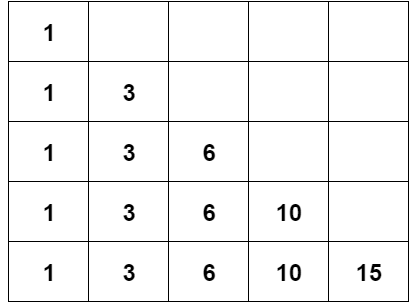
\includegraphics[scale=0.5]{table.png}
  \caption{Przykładowa tabela stworzona przez algorytm dla żółwi o wartościach (waga, wytrzymałość): (1,1) (2,3) (3,6) (4,10) (5,15). 
Widać, że z podanych żółwi możemy zbudować tron o wysokości 5 i wadze 15. }
  \label{fig:table1}
\end{figure}

Każda kolejna iteracja algorytmu to kolejny wiersz tabeli. Do każdej kolejnej kolumny tabeli wpisywana jest wartość minimalna z porównania:
\begin{lstlisting}
min(table[i][j], table[i - 1][j])
\end{lstlisting}
Jeśli żółw może udźwignąć wartość z poprzedniej iteracji, to w aktualne pole wybieramy: 
\begin{lstlisting}
min(table[i][j], table[i-1][j-1]+turtles[i].getWeight())
\end{lstlisting}
gdzie i, j to odpowiednio aktualny wiersz i kolumna, a turtles[i] to aktualnie rozpatrywany żółw.

\subsubsection{Kod}
\begin{lstlisting}
table[0][1] = turtles[0].getWeight();
for (unsigned int i = 1; i < N; ++i)
{
  for (unsigned int j = 1; j <= i + 1; ++j)
  {
    table[i][j] = min(table[i][j], table[i - 1][j]);
    if (turtles[i].getCapacity() >= table[i - 1][j - 1])
    {
      table[i][j] = min(table[i][j],
                        table[i - 1][j - 1]+turtles[i].getWeight());
    }
  }
}

// looking for index of last element in last row(height of Throne)
for (unsigned int i = N; i >= 0; --i)
{
  if (table[N - 1][i] != numeric_limits<unsigned int>::max())
  {
    return i;
  }
}
\end{lstlisting}


\subsection{Algorytm naiwny}
\subsubsection{Złożoność}
Złożoność asymptotyczna wynosi 
\begin{equation}
O(n^2)
\end{equation}
Złożoność dokładna wynosi w przybliżeniu:
\begin{equation}
T(n)=n^2+n
\end{equation}

\subsubsection{Opis}
Złożoność
Rozwiązanie polega na przejściu w pętli tyle razy ile jest żółwi, za każdym razem wybierając najlżejszego żółwia(jeśli żółwie mają taką samą wagę, to wybieramy żółwia z mniejszą wytrzymałością). Znalezionego żółwia następnie umieszczamy na stos pod warunkiem, że jest w stanie go unieść. Jeśli żółw, który jest w danej chwili na szczycie stosu może unieść więcej niż aktualnie znaleziony żółw i da radę unieść także nowego, to zostaje on na szczycie stosu, a pod niego wkłada się nowego żółwia.
\subsubsection{Kod}
\begin{lstlisting}
// putting first turtle on stack
auto firstTurtle = min_element(turtles.begin(), turtles.end());

// if there are no turtles in vector, return 0	
if (firstTurtle == turtles.end())
	return 0;

unsigned int stackWeight = firstTurtle->getWeight(); 
unsigned int stackHeight = 1;

Turtle lastTurtle = *firstTurtle;

// erase first turtle from vector
turtles.erase(firstTurtle);

for (int i = 0; i < turtles.size(); ++i)
{
  // looking for the lightest turtle
  auto it = min_element(turtles.begin(), turtles.end());
	
  // if lastTurtle in stack has got better capacity than turtle 
  // that we found and new turtle can hold stack - 
  // we can maybe swap them on the top of stack		
  if (lastTurtle.getCapacity() > it->getCapacity() 
    && it->getCapacity() >= stackWeight)						
  {
    // if lastTurtle can hold the stack with new turtle
    if(lastTurtle.getStrength() > stackWeight + it->getWeight())	
    {
      stackWeight += it->getWeight();
      ++stackHeight;
			
      // erasing current turtle from vector
      turtles.erase(it);	
      continue;
     }
  }
	
  // if new turtle can hold current stack - push it on it
  if (it->getCapacity() >= stackWeight)	
  {
    ++stackHeight;
    stackWeight += it->getWeight();
    lastTurtle = *it;
  }
	
  // erasing current turtle from vector
  turtles.erase(it);	
}

return stackHeight;
\end{lstlisting}

\subsection{Algorytm z presortowaniem}
\subsubsection{Złożoność}
Złożoność asymptotyczna wynosi 
\begin{equation}
O(nlog_2(n))
\end{equation}
Złożoność dokładna wynosi w przybliżeniu:
\begin{equation}
T(n)=nlog_2(n)+n
\end{equation}
\subsubsection{Opis}
Algorytm bardzo przypomina przedstawione powyżej podejście naiwne. Na samym początku kolekcja żółwi jest sortowana według wagi. Następnie algorytm przechodzi po wszystkich żółwiach w pętli i próbuje je wrzucać na stos(sprawdzanie czy można wrzucić na stos jest analogiczne do algorytmu naiwnego).

\subsubsection{Kod}
\begin{lstlisting}
sort(turtles.begin(), turtles.end());

unsigned int stackWeight = 0, stackHeight = 0;
auto lastTurtle = turtles.begin();
for (auto it = turtles.begin(); it != turtles.end(); ++it)
{
  if (lastTurtle->getCapacity() > it->getCapacity() 
    && it->getCapacity() >= stackWeight)
  {
      if (lastTurtle->getStrength() > stackWeight + it->getWeight() )
      {
        stackWeight += it->getWeight();
        ++stackHeight;
        continue;
      }
			
    }
    if (it->getCapacity() >= stackWeight)
    {
      ++stackHeight;
      stackWeight += it->getWeight();
      lastTurtle = it;
    }
}
return stackHeight;
\end{lstlisting}

\section{Moduły źródłowe}
Program został podzielony na następujące moduły:
\begin{description}
	\item[ResultsTable] \hfill \\ 
	Klasa tworząca tabelkę z wynikami. Posiada metodę, która po podaniu do niej jako argument jednej z klas dziedziczących po Throne, generuje żółwie, wywołuje algorytm rozwiązujący problem oraz zapamiętuje czas jego wykonania. Funkcja iteruje po kilku rozmiarach problemu i następnie rysuje w konsoli tabelkę.
	
	\item[Throne] \hfill \\  
	Klasa abstrakcyjna przechowująca zbiór żółwi. Umożliwia ich generowanie oraz posiadaja metodę do rozwiązania problemu. Funkcja, która rozwiązuje problem jest czysto wirtualna i powinna być dostarczona przez klasy potomne. Klasa implementuje generator żółwi, który generuje je z rozkładu jednostajnego(rozkład został wybrany metodą prób i błędów. Zwracane przez niego dane umożliwiały zbudowanie najwyższej wieży. Rozkład normalny dawał podobne wyniki, ale odrobinę gorsze).
	
	\item[ThroneDynamicProgramming] \hfill \\ 
	 Klasa dziedzicząca po Throne, rozwiązuje problem za pomocą programowania dynamicznego.
	 
	\item[ThroneFast] \hfill \\ 
	 Klasa dziedzicząca po Throne, rozwiązuje problem w najszybszy sposób.
	 
	\item[ThroneNaive] \hfill \\  
	 Klasa dziedzicząca po Throne, rozwiązuje problem za pomocą algorytmu naiwnego.
	 
	\item[Timer] \hfill \\ 
	 Singleton, klasa timera odmierzającego czas, wykorzystywanego do sprawdzenia czasu wykonania algorytmów. Czas jest odliczany w nanosekundach.
	 
	\item[Turtle] \hfill \\ 
	 Klasa reprezentująca pojedynczego żółwia posiadającego atrybuty takie jak waga i wytrzymałość.
\end{description}

\section{Przykładowe wyniki pomiarów czasu}
\subsection{Programowanie dynamiczne}
Algorytm programowania dynamicznego działa z kwadratową złożonością. Ma również dużą złożoność pamięciową, ponieważ alokuje tablicę o rozmiarze NxN, gdzie N to liczba żółwi. W algorytmie zastosowano małą optymalizację, dzięki czemu zmniejszono rozmiar tablicy o około połowę(zaalokowano dolną połówkę tablicy, ponieważ wartości powyżej jej przekątnej są nieistotne, można to zauważyć na rysunku \ref{fig:table1}). Algorytm działa w podobnym czasie jak algorytm naiwny.

\begin{figure}[h]
  \centering
  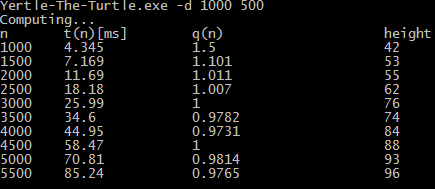
\includegraphics[scale=1.25]{yertleD.png}
  \caption{Przykładowe wykonanie programu dla algorytmu programowania dynamicznego, przy początkowym rozmiarze problemu 1000 i kolejnych iteracjach co 500 }
  \label{fig:yertleD}
\end{figure}

\newpage
\subsection{Algorytm naiwny}
Algorytm naiwny działa z kwadratową złożonością. Ma jednak o wiele mniejszą złożoność pamięciową. Czas jego wykonania jest bardzo podobny do czasu wykonania algorytmu korzystającego z programowania dynamicznego.

\begin{figure}[h]
  \centering
  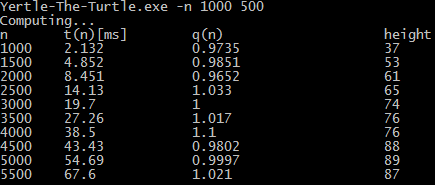
\includegraphics[scale=1.25]{yertleN.png}
  \caption{Przykładowe wykonanie programu dla algorytmu naiwnego, przy początkowym rozmiarze problemu 1000 i kolejnych iteracjach co 500 }
  \label{fig:yertleN}
\end{figure}

\section{Algorytm z presortowaniem}
Algorytm wykonuje się zdecydowanie najszybciej, różnica wynosi około 2 rzędy wielkości w stosunku do pozostałych dwóch algorytmów.
\begin{figure}[h]
  \centering
  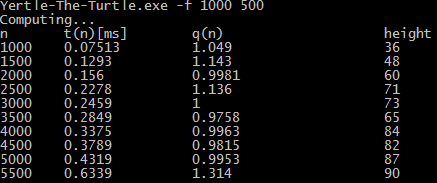
\includegraphics[scale=1.25]{yertleF.png}
  \caption{Przykładowe wykonanie programu dla algorytmu z presortowaniem, przy początkowym rozmiarze problemu 1000 i kolejnych iteracjach co 500 }
  \label{fig:yertleF}
\end{figure}





\end{document}
